\documentclass[12pt]{article} 

\usepackage{fullpage}
\usepackage{bookmark}
\usepackage{amsmath}
\usepackage{amssymb}
\usepackage[dvipsnames]{xcolor}
\usepackage{hyperref} % for the URL
\usepackage[shortlabels]{enumitem}
\usepackage{mathtools}
\usepackage[most]{tcolorbox}
\usepackage[amsmath,standard,thmmarks]{ntheorem} 
\usepackage{physics}
\usepackage{pst-tree} % for the trees
\usepackage{verbatim} % for comments, for version control
\usepackage{tabu}
\usepackage{tikz}
\usepackage{float}
\usepackage{siunitx}
\usepackage{physunits}

% From the Plot video

\usepackage[LGR,T1]{fontenc}
\usepackage[utf8]{inputenc}
\usepackage{lmodern}
\usepackage{microtype}
\usepackage{upgreek}
\usepackage[misc]{ifsym}

\usepackage{pgfplots}
	\usetikzlibrary{
		calc,
		patterns,
		positioning
	}
	\pgfplotsset{
		compat=1.16,
		samples=200,
		clip=false,
		my axis style/.style={
			axis x line=middle,
			axis y line=middle,
			legend pos=outer north east,
			axis line style={
				->,
			},
			legend style={
				font=\footnotesize
			},
			label style={
				font=\footnotesize
			},
			tick label style={
				font=\footnotesize
			},
			xlabel style={
				at={
					(ticklabel* cs:1)
				},
				anchor=west,
				font=\footnotesize,
			},
			ylabel style={
				at={
					(ticklabel* cs:1)
				},
				anchor=west,
				font=\footnotesize,
			},
			xlabel=$t$,
			ylabel=$\vec d(\m \tx{[East]})$
		},
	}
	\tikzset{
		>=stealth
	}


    \pgfplotsset{my style/.append style={axis x line=middle, axis y line=
           middle, xlabel={$t$}, axis equal }}

%%% Tables and figures packages

\usepackage{float}
\usepackage{caption}
	\captionsetup{
		format=plain,
		labelfont=bf,
		font=small,
		justification=centering
	}
	
%%% Numbers and sets

\newcommand{\E}{\mathrm{e}}
\newcommand{\tx}[1]{\text{#1}}


% floor, ceiling, set
\DeclarePairedDelimiter{\ceil}{\lceil}{\rceil}
\DeclarePairedDelimiter{\floor}{\lfloor}{\rfloor}
\DeclarePairedDelimiter{\set}{\lbrace}{\rbrace}
\DeclarePairedDelimiter{\iprod}{\langle}{\rangle}

\DeclareMathOperator{\Int}{int}
\DeclareMathOperator{\mean}{mean}

% commonly used sets
\newcommand{\R}{\mathbb{R}}
\newcommand{\Nat}{\mathbb{N}}
\newcommand{\Q}{\mathbb{Q}}
\renewcommand{\P}{\mathbb{P}}

\newcommand{\sset}{\subseteq}


\theoremstyle{break}
\theorembodyfont{\upshape}

\newtheorem{thm}{Theorem}[subsection]
\tcolorboxenvironment{thm}{
enhanced jigsaw,
colframe=Dandelion,
colback=White!90!Dandelion,
drop fuzzy shadow east,
rightrule=2mm,
sharp corners,
before skip=10pt,after skip=10pt
}

\newtheorem{cor}{Corollary}[thm]
\tcolorboxenvironment{cor}{
boxrule=0pt,
boxsep=0pt,
colback={White!90!RoyalPurple},
enhanced jigsaw,
borderline west={2pt}{0pt}{RoyalPurple},
sharp corners,
before skip=10pt,
after skip=10pt,
breakable
}

\newtheorem{algo}[thm]{Algorithm}
\tcolorboxenvironment{algo}{
enhanced jigsaw,
colframe=Red,
colback={White!95!Red},
rightrule=2mm,
sharp corners,
before skip=10pt,after skip=10pt
}

\newtheorem{ex}[thm]{Example}
\tcolorboxenvironment{ex}{% from ntheorem
blanker,left=5mm,
sharp corners,
before skip=10pt,after skip=10pt,
borderline west={2pt}{0pt}{Green}
}

\newtheorem*{pf}{Proof}
\tcolorboxenvironment{pf}{% from ntheorem
breakable,blanker,left=5mm,
sharp corners,
before skip=10pt,after skip=10pt,
borderline west={2pt}{0pt}{NavyBlue!80!white}
}


\newtheorem*{soln}{Solution}
\tcolorboxenvironment{soln}{% from ntheorem
breakable,blanker,left=5mm,
sharp corners,
before skip=10pt,after skip=10pt,
borderline west={2pt}{0pt}{NavyBlue!80!white}
}

\newtheorem{defn}{Definition}[subsection]
\tcolorboxenvironment{defn}{
enhanced jigsaw,
colframe=Cerulean,
colback=White!90!Cerulean,
drop fuzzy shadow east,
rightrule=2mm,
sharp corners,
before skip=10pt,after skip=10pt
}

\newtheorem{prop}[thm]{Proposition}
\tcolorboxenvironment{prop}{
boxrule=0pt,
boxsep=0pt,
colback={White!90!Green},
enhanced jigsaw,
borderline west={2pt}{0pt}{Green},
sharp corners,
before skip=10pt,
after skip=10pt,
breakable
}

\setlength\parindent{0pt}
\setlength{\parskip}{2pt}


\begin{document}
\let\ref\Cref
\section{Speed and Velocity}
\subsection{Average Speed}

\begin{defn}
The \textbf{average speed} of an object is the ratio of the total distance traveled to the time elapsed. 
$$v_{av} = \frac{d}{\Delta t}$$
Here $\Delta t = t_f - t_i$, or in other words the elapsed time.
\end{defn}
We can conclude of course that $v_{av}$ is of course a \emph{scalar}, it has no associated direction, you could also argue that it is the ratio of two scalar quantities, time and distance, and hence it must be a scalar. The average speed is a common quantity we encounter everyday. Over a given distance traversed, our speed varies quite often, the average speed tells us the most common speed we were traveling at throughout the journey. \\


\textbf{Remark:} The units of $v_{av}$ are the units of $d$ divided by the units of $\Delta t$. (m /s for example).
\begin{ex}
I am currently at the Library, $500\m$[East] relative to my home. I decide to walk $350\m$[West] to the Store. Compute my average speed if the trip took an hour. (In m/s)
\end{ex}
\begin{soln}
$\implies$
    \vspace*{9cm}
\end{soln}
   \newpage 

\subsection{Average Velocity}
    
\begin{defn}
    The \textbf{average velocity} of an object is the ratio of the displacement to the time elapsed
    $$\vec v_{av} = \frac{\overrightarrow{\Delta d}}{\Delta t}$$
\end{defn}
We can conclude that $\vec v_{av}$ is a \emph{vector quantity}, this is true because we can think of$(1 / \Delta t)$ as a scalar, and a scalar multiplied by a vector ($\overrightarrow{\Delta d})$ is always a vector. The average velocity cares about our final position vector as well as our initial position vector.

\begin{ex}
    I am currently at the Library, $500\m$[East] relative to my home. I decide to walk $350\m$[West] to the Store. Compute my average \emph{velocity} if the trip took an hour.
\end{ex}
\begin{soln}
$\implies$
    \vspace*{10cm}
\end{soln}



\newpage

\begin{defn}
    A \textbf{position-time graph} is a graph of position versus time. We plot a set of position vectors on the vertical axes with their corresponding time on the horizontal axes. 
\end{defn}
For example let us consider a simple position versus time graph for a Ball rolling across a road starting at coordinates (0,0). 
\begin{figure}[h]
	\centering
	\begin{tikzpicture}
	\begin{axis}[
		my axis style,
		width=0.5\textwidth,
		height=.5\textwidth,
        xlabel=$t$,
		ylabel=$\vec d (\m \tx{[East]})$
	]
	
	\addplot[
		domain=0:4,
		thick,
		-
	]
	{x};
	
	\fill[
		black
	];
	
	\end{axis}
	\end{tikzpicture}
	\caption{Position V. Time}
	\label{fig:my-awesome-graph}
\end{figure}

At various time intervals, we can immediately extract the position of the Ball relative to the reference point (0,0). For example, at $t = 3$, the balls position vector was $\vec d = 3\m$[East].\\

\textbf{Remark: } Note that this graph assigns [East] as the positive direction of motion, this is because all points on the vertical axes are positive.


We can also consider the case of the Ball travelling [West] starting fom (0,0). We give the graph below,


\begin{center}
\begin{tikzpicture}
    \begin{axis}[my style]
         \addplot[domain=0:4] {-x};
    \end{axis}
\end{tikzpicture}
\end{center}



\begin{center}
\textbf{Figure 2 :} Position V. Time (West case)
\end{center}

\begin{ex}
I start at the Shopping center, $500\m$[Right] of my house. I then travel $240\m$[Left] to the Library. Preform the following,
\begin{enumerate}[label=(\alph*)]
	\item Draw the Graph of the trip.
	\item Compute my average speed
	\item Compute my average velocity
\end{enumerate}
\end{ex}
\begin{soln}
	$\implies$
	\vspace*{5cm}
\end{soln}
\newpage

\newpage
\vspace*{8cm}

\subsection{Motion with Uniform and Non-uniform velocity}
\begin{defn}
	\textbf{Uniform motion} (Or constant velocity) is motion where the velocity is fixed.
\end{defn}
Uniform motion has some unique properties which we will uncover later on and is hence important to make mention of. We usually encounter constant velocity motion on the road, is it true that you (or the driver) is always in a state of acceleration (changing velocity)?
\begin{defn}
	\textbf{Non-uniform motion} (Or accelerated motion) is motion where the velocity is \emph{not} fixed.
\end{defn}

\begin{prop}
Given a $\textbf{Linear}$ Position v. Time plot of a moving body, the slope $m$ represents the average velocity of the body.
\end{prop}
\begin{pf}
Let the slope of the Position v. Time graph be $m$, let us compute this slope by using the slope formula, namely,
$$m = \frac{y_2 - y_1}{x_2 - x_1}$$
Since the $y-$coordinates on a Position v. Time graph are position vectors $\vec d$, and the $x-$coordinates are time points, $t$, we can translate this slope formula to the equivalent,
$$m = \frac{\vec d_2 - \vec d_1}{t_2 - t_1}$$
At this point we are free to choose any two coordinate pairs $(\vec d_1,t_1)$, $(\vec d_2, t_2)$, let us choose $(\vec d_f, t_f)$, $(\vec d_i, t_i)$, the final and initial coordinate pairs of the moving body. This gives,
$$m = \frac{\vec d_f - \vec d_i}{t_f - t_i} = \vec v_{av}$$
 \qed
\end{pf}


\subsection{Being fluent in proofs}
I want to stress the importance of being fluent in proofs. Although this is rather mathematical, much of the concepts we will come across in physics are described mathematically and understanding them at a mathematical level will enable us to comprehend the material that much better, this is especially important for higher level physics and is why many mathematicians can grasp higher level physics that much easier. Now being able to prove a given proposition not only demonstrates your understanding of such a concept, but allows you to unveil alternative observations that may be of use.



\subsection{Types of motion from Position v. Time Plots}
In this course we will encounter common types of motion and hence it would be useful to make mention of their plots and what they look like, as this should in turn enhance the students comprehension of the particular motion they are dealing with.

\begin{enumerate}[label = (\alph*)]
	\item 
        \begin{tikzpicture}
        \begin{axis}[
            my axis style,
            width=\textwidth,
            height=.5\textwidth,
        ]
        
        \addplot[
            domain=0:5,
            thick,
            purple,
            -
        ]
        {2};
    
        \fill[
            black
        ];
        
        \end{axis}
        \end{tikzpicture}
		
		\textbf{\large{Properties of type (a):}}
		\begin{itemize}
			\item The slope of the graph is zero, hence $\vec v_{av} = +0\m / \s$.
			\item The object is at \textbf{rest}.
			\item The object is [East] relative to the reference point (0,0).
		\end{itemize}


	\item 
	\begin{tikzpicture}
        \begin{axis}[
            my axis style,
            width=\textwidth,
            height=.5\textwidth,
			ylabel = $ $,
        ]
        
        \addplot[
            domain=0:5,
            thick,
            purple,
            -
        ]
        {-2};
    
        \fill[
            black
        ];
        
        \end{axis}
        \end{tikzpicture}
		
		\textbf{\large{Properties of type (b):}}
		\begin{itemize}
			\item The slope of the graph is zero, hence $\vec v_{av} = +0\m / \s$.
			\item The object is at \textbf{rest}.
			\item The object is [West] relative to the reference point (0,0).
		\end{itemize}


	\item 
	\begin{tikzpicture}
        \begin{axis}[
            my axis style,
            width=\textwidth,
            height=.5\textwidth,
        ]
        
        \addplot[
            domain=0:5,
            thick,
            purple,
            -
        ]
        {2*x};

		\addplot[
		domain=0:2,
		thick,
		blue,
		dashdotted,
		]
		{4};

		\draw [dashed, blue, thick] (2,0) -- (2,4);
    
        \fill[
            black
        ];
        
        \end{axis}
        \end{tikzpicture}
		
		\textbf{\large{Properties of type (c):}}
		\begin{itemize}
			\item The slope of the graph is $m = +2$, hence $\vec v_{av} = +2\m / \s$.
			\item The object experiencing \textbf{uniform motion} or \textbf{constant velocity}.
			\item The object is traveling in the [East] direction.
		\end{itemize}

	\item 
	\begin{tikzpicture}
        \begin{axis}[
            my axis style,
            width=\textwidth,
            height=.5\textwidth,
        ]
        
        \addplot[
            domain=0:5,
            thick,
            purple,
            -
        ]
        {-2*x + 10};

		\addplot[
		domain=0:3,
		thick,
		blue,
		dashdotted,
		]
		{4};

		
		\draw [dashed, blue, thick] (3,0) -- (3,4);
    
        \fill[
            black
        ];
        
        \end{axis}
        \end{tikzpicture}
		
		\textbf{\large{Properties of type (d):}}
		\begin{itemize}
			\item The slope of the graph is $m = -2$, hence $\vec v_{av} = -2\m / \s$.
			\item The object experiencing \textbf{uniform motion} or \textbf{constant velocity}.
			\item The object is traveling in the [West] direction.
		\end{itemize}

\end{enumerate}


\begin{ex}
    Given the position v. time plot below, determine the following,

    \begin{enumerate} [label = (\alph*)]
        \item Determine the average velocity and the average speed from over the first $4$ seconds.
        \item Are the results from the (a) the same if instead I asked you to compute the result from $t_1 = 2 \rightarrow t_2 = 4$
    \end{enumerate}

    \begin{center}
    \begin{tikzpicture}
    \begin{axis}[my style]
         \addplot[domain=0:4] {x};
    \end{axis}
    \end{tikzpicture}
    \end{center}

\end{ex}

\begin{soln}
$\implies$
\vspace*{7cm}

\end{soln}
\textbf{\large{1.5 \hspace*{0.2cm} Plots with equations}}\\
Sometimes it is more convenient to represent the equation of a position v. time plot by a standard mathematical equation, $y = 2x$ for example. However since we are almost always dealing with the variable $t$ along the horizontal axes we are unable to use $x$, instead we must replace $x \rightarrow t$. Since $y$ always corresponds to vertical motion, we would like to preserve the fact that $x$ represents horizontal motion, hence when plotting pos v.time plots we represent the position vector by the variable $x$. Hence the equation $y = x$ translated to a pos v. time plot would be $x = t$. 

\textbf{Remark: }All motion above the horizontal axes is called the positive direction direction of motion, we also assume that we are working with the $x-$dimensional coordinate system.
\begin{ex} 
	Three runners compete in a race, Dave, Thomas and Ryan. Listed below are their equations of motion, if the race lasted $5$ minutes, determine who won the race.
	\begin{itemize}
		\item \textcolor{orange}{Ryan} $\colon x_R = 2t$
		\item \textcolor{blue}{Dave} $\colon x_D = 3t$
		\item \textcolor{red}{Thomas} $\colon x_T = t$
	\end{itemize}
\end{ex}
\begin{soln}
	$\implies$
	\begin{center}
		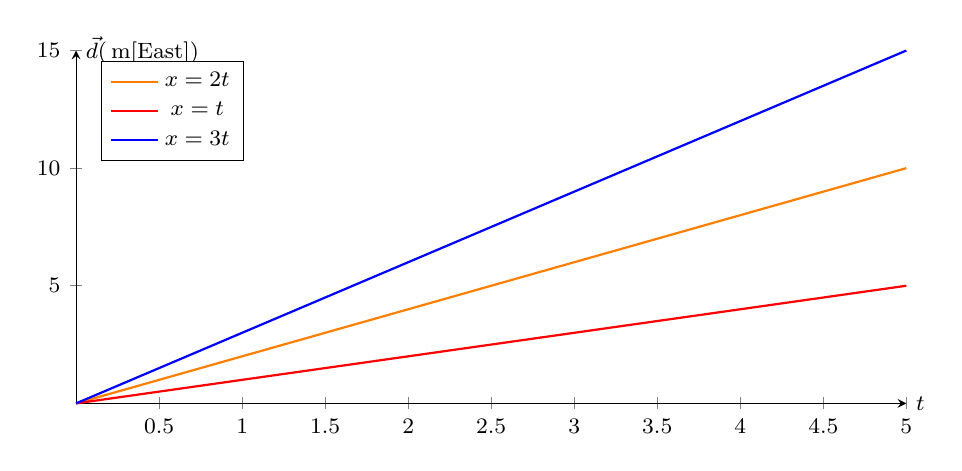
\begin{tikzpicture}
			\begin{axis}[
				my axis style,
				width=\textwidth,
				height=.5\textwidth,
				legend entries={
					$x = 2t$,
					$x = t$,
					$x = 3t$
				},
				legend pos=north west
			]
			
			\addplot[
				domain=0:5,
				thick,
				orange,
				-
			]
			{2*x};
		
			\addplot[
				domain=0:5,
				thick,
				red,
				-
			]
			{(x)};
		
			\addplot[
				domain=0:5,
				thick,
				blue,
				-
			]
			{3*(x)};
			
			\fill[
				black
			];
			
			\end{axis}
		\end{tikzpicture}
		\end{center}
		(continued)
\vspace*{15cm}
\end{soln}
\textbf{\large{1.6 An important note about Calculations}}\\
Unlike mathematics, in physics we care about the units in our calculations. This is because during operations of arithmetic with numbers from physics, we must ensure that the units are compatible. For example, if we are preforming arithmetic with two distance values, we must ensure that they share the same units. When it comes to operations with velocity or acceleration values, then we must ensure that both the [time] units as well as the units of [distance] are compatible.
\newpage 
\begin{ex}
	A racecar clears a $1\km$ track at speed of $500 \m / \s$. Compute the time he took to clear the track in seconds. 
\end{ex}
\begin{soln}
$\implies$
\vspace*{4cm}
\end{soln}



\end{document}
